\documentclass{article}
\usepackage[final]{nips_2017}
\usepackage{polski}
\usepackage[utf8]{inputenc}    % allow utf-8 input
\usepackage[T1]{fontenc}       % use 8-bit T1 fonts
\usepackage{hyperref}          % hyperlinks
\usepackage{url}               % simple URL typesetting
\usepackage{booktabs}          % professional-quality tables
\usepackage{amsfonts}          % blackboard math symbols
\usepackage{nicefrac}          % compact symbols for 1/2, etc.
\usepackage{microtype}         % microtypography
\usepackage[section]{placeins} % figures kept in sections
\usepackage{graphicx}          % images
\graphicspath{ {./img/} }
\usepackage{multirow}
\usepackage{float}             % figures in place
\usepackage{caption}		   % smaller margin after figure

\renewcommand{\figurename}{Wykres}
\setlength{\belowcaptionskip}{-20pt}

\title{  Regularyzacja\\Sieci Neuronowe 2020 }

\author{
  Jakub Ciszek \\
  238035\\
}

\begin{document}

\maketitle

\newpage
\tableofcontents
\newpage

Cały kod wykorzystany w zadaniu znajduje się pod adresem: \url{https://github.com/Greenpp/sieci-neuronowe-pwr-2020}

\section{Opis badań}
\subsection{Plan eksperymentów}

Wszystkie eksperymenty zostały przeprowadzone 10 razy. Losowość przy inicjalizacji wag oraz generacji danych nie została narzucona żadnym ziarnem. Podczas badań przyjęto górną granicę 40 epok, po przekroczeniu której, uczenie zostawało przerywane. Ze względu na charakter zadania (klasyfikacja) na ostatniej warstwie użyto funkcji Softmax, a za funkcję straty przyjęto Entropię krzyżową. Sieć posiadała jedną warstwę ukrytą, złożoną z 512 neuronów. Za funkcję aktywacyjną posłużyła ReLU, wagi zostały wylosowane z przedziału \($-0.1 -- 0.1$\). W celu przyspieszenia procesu uczenia do aktualizacji parametrów użyto metody Adam.
W procesie uczenia użyto paczek wielkości 1024 elementów.\\
Zostały przeprowadzone następujące badania:
\begin{itemize}
	\item Wpływ dropoutu na przebieg procesu uczenia.
	\item Wpływ regularyzacji L1 na przebieg procesu uczenia.
	\item Wpływ regularyzacji L2 na przebieg procesu uczenia.
	\item Wpływ regularyzacji łączonej L1 i L2 na przebieg procesu uczenia.
	\item Porównanie metod.
\end{itemize}
Podczas wizualizacji funkcji straty pominięto pierwsze 10 pomiarów dla lepszej czytelności.

\subsection{Charakterystyka zbiorów danych}

Danymi użytymi w zadaniu jest zbiór ręcznie pisanych cyfr \(0-9\) - MNIST. Na zbiór składa się 70,000 obrazów wielkości 28x28 pikseli, co po przekształceniu odpowiadało 784 elementowemu wektorowi wejściowemu i 10 klasom na wyjściu. Użyta w zadaniu wersja została podzielona na 3 zbiory:
\begin{itemize}
	\item Uczący - 50,000 przykładów.
	\item Walidujący - 10,000 przykładów.
	\item Testowy - 10,000 przykładów.
\end{itemize}
W trakcie eksperymentów wykorzystano jedynie pierwsze 10,000 przykładów zbioru uczącego i testowy. Zbiór uczący został ograniczony aby łatwiej pokazać wpływ regularyzacji na przeuczenie.

\newpage
\section{Eksperymenty}

\subsection{Wpływ dropoutu na przebieg procesu uczenia}
\subsubsection*{Założenia}
\begin{table}[H]
	\caption{Stałe dla eksperymentu 1}
	\label{tabela-const-1}
	\centering
	\begin{tabular}{lr}
		\toprule
		Parametr      & Wartość \\
		\midrule
		Regularyzacja & Dropout   \\
		\bottomrule
	\end{tabular}
\end{table}

Zmienną w tym eksperymencie była szansa na wyłączenie połączenia. Prawdopodobieństwo przyjmowało wartości ze zbioru \(\{$0.0, 0.2, 0.5, 0.8$\}\)
\subsubsection*{Przebieg}

Podczas eksperymentu model został zainicjalizowany 10 razy dla każdej z badanych wartości oraz wyuczony, uzyskane wyniki zostały zapisane w postaci pliku .plk do dalszej analizy.

\subsubsection*{Wyniki}
\begin{figure}[H]
	\centering
	\caption{Dokładność modelu w zależności od prawdopodobieństwa wyłączenia połączenia}
	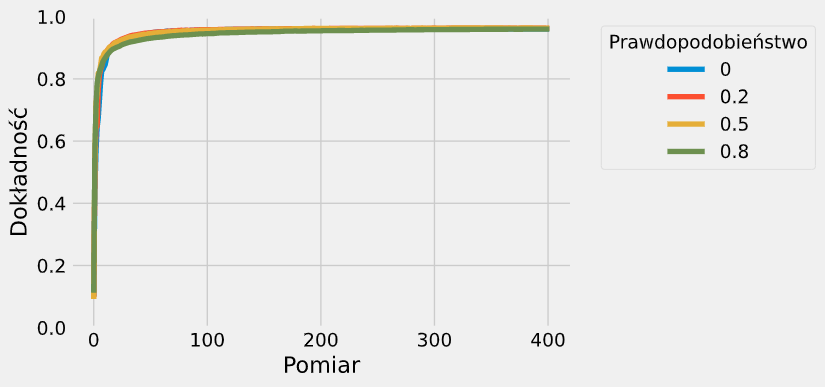
\includegraphics[width=\textwidth]{drop_acc.png}
	\label{fig:res11}
\end{figure}
\begin{figure}[H]
	\centering
	\caption{Dokładność modelu w końcowym etapie uczenia w zależności od prawdopodobieństwa wyłączenia połączenia}
	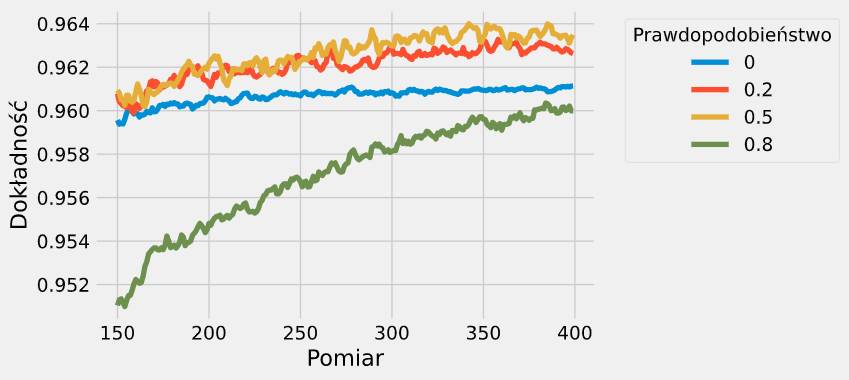
\includegraphics[width=\textwidth]{drop_acc_zoom.png}
	\label{fig:res12}
\end{figure}
\begin{figure}[H]
	\centering
	\caption{Zachowanie funkcji błędu dla prawdopodobieństwa 0.0}
	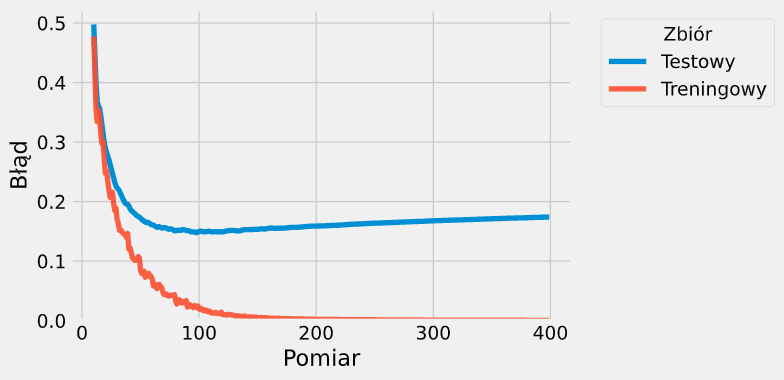
\includegraphics[width=\textwidth]{drop_err_0.png}
	\label{fig:res13}
\end{figure}
\begin{figure}[H]
	\centering
	\caption{Zachowanie funkcji błędu dla prawdopodobieństwa 0.2}
	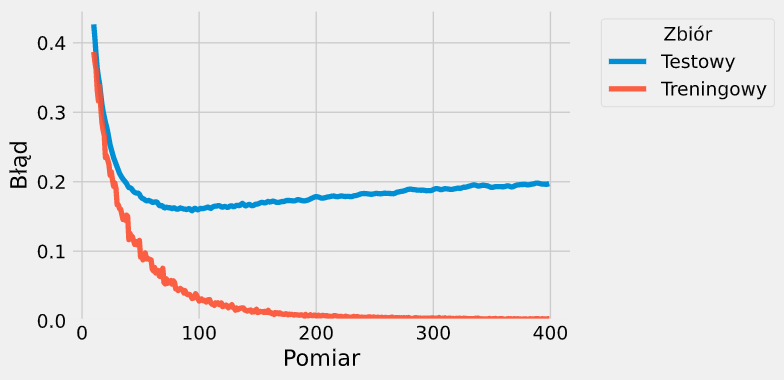
\includegraphics[width=\textwidth]{drop_err_02.png}
	\label{fig:res14}
\end{figure}
\begin{figure}[H]
	\centering
	\caption{Zachowanie funkcji błędu dla prawdopodobieństwa 0.5}
	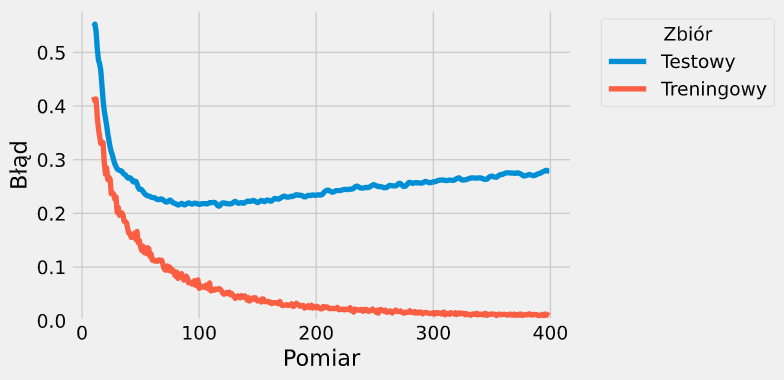
\includegraphics[width=\textwidth]{drop_err_05.png}
	\label{fig:res15}
\end{figure}
\begin{figure}[H]
	\centering
	\caption{Zachowanie funkcji błędu dla prawdopodobieństwa 0.8}
	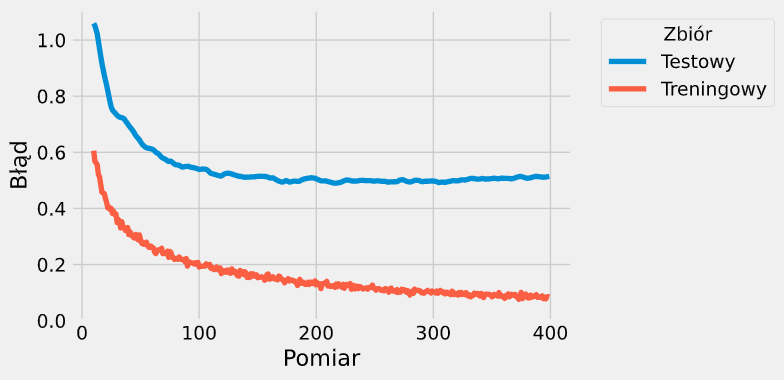
\includegraphics[width=\textwidth]{drop_err_08.png}
	\label{fig:res16}
\end{figure}

\begin{table}[H]
	\caption{TODO}
	\label{tabela-res-11}
	\centering
	\begin{tabular}{rrr}
		\toprule
		Prawdopodobieństwo & Dokładność [\%] \\
		\midrule
		0.0                 & 96.17              \\
		0.2                 & 96.45              \\
		0.5                 & \textbf{96.58}     \\
		0.8                 & 96.14              \\
		\bottomrule
	\end{tabular}
\end{table}

\subsubsection*{Wnioski}
Na przedstawionych wykresach~\ref{fig:res11},~\ref{fig:res12} oraz tabeli~\ref{tabela-res-11} można zauważyć, że dokładność modelu nie zmieniła się znacznie, niezależnie od prawdopodobieństwa z jakim połączenia były wyłączane. Zauważalnym efektem jest natomiast zanikający efekt przeuczenia, widoczny na wykresach~\ref{fig:res13},~\ref{fig:res14} i~\ref{fig:res15}, widoczny na wykresie~\ref{fig:res16}, przy wyłączeniu 80\% połączeń, gdzie błąd treningowy nie spada tak blisko 0 jak w pozostałych przypadkach, a błąd testowy nie rośnie tak gwałtownie.

\newpage
\subsection{Wpływ regularyzacji L1 na przebieg procesu uczenia}
\subsubsection*{Założenia}
\begin{table}[H]
	\caption{Stałe dla eksperymentu 2}
	\label{tabela-const-2}
	\centering
	\begin{tabular}{lr}
		\toprule
		Parametr      & Wartość \\
		\midrule
		Regularyzacja & L1        \\
		Lambda        & 0.0001    \\
		\bottomrule
	\end{tabular}
\end{table}

\subsubsection*{Przebieg}

Podczas eksperymentu model został zainicjalizowany 10 razy dla każdej z badanych wartości oraz wyuczony, uzyskane wyniki zostały zapisane w postaci pliku .plk do dalszej analizy.

\subsubsection*{Wyniki}
\begin{figure}[H]
	\centering
	\caption{Zachowanie funkcji błędu bez regularyzacji}
	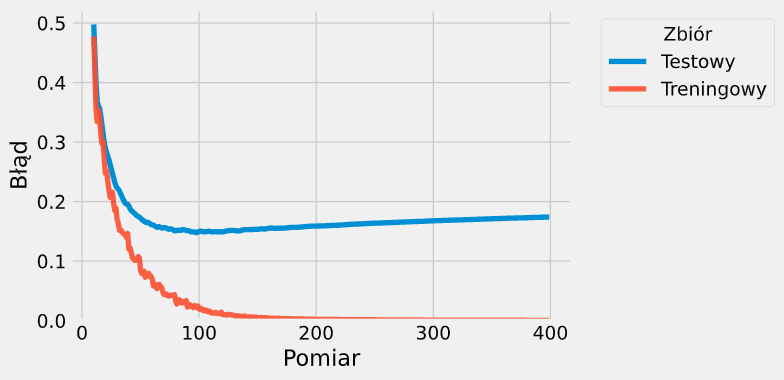
\includegraphics[width=\textwidth]{drop_err_0.png}
	\label{fig:res21}
\end{figure}
\begin{figure}[H]
	\centering
	\caption{Zachowanie funkcji błędu dla regularyzacji L1}
	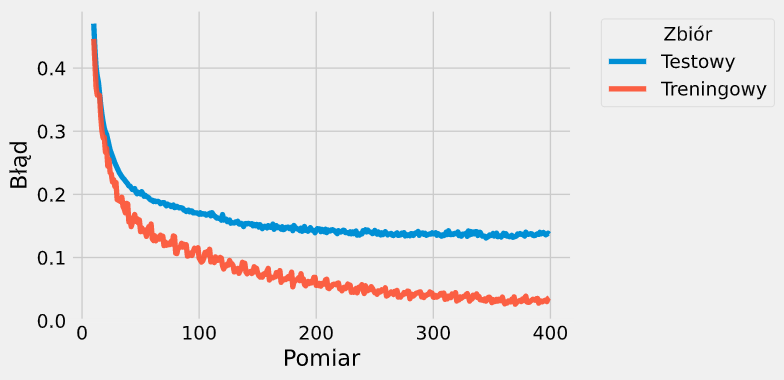
\includegraphics[width=\textwidth]{reg_err_l1.png}
	\label{fig:res22}
\end{figure}



\subsubsection*{Wnioski}
Na przedstawionym wykresie~\ref{fig:res22} można zaobserwować eliminację problemu przeuczenia, zaobserwowanego przy uczeniu bez regularyzacji (wykres~\ref{fig:res21}). Błąd testowy w przeprowadzonym eksperymencie nie przestaje spadać, a błąd treningowy nie osiąga 0, co sugeruje lepszą generalizację.

\newpage
\subsection{Wpływ regularyzacji L2 na przebieg procesu uczenia}
\subsubsection*{Założenia}
\begin{table}[H]
	\caption{Stałe dla eksperymentu 3}
	\label{tabela-const-3}
	\centering
	\begin{tabular}{lr}
		\toprule
		Parametr      & Wartość \\
		\midrule
		Regularyzacja & L2        \\
		Lambda        & 0.0001    \\
		\bottomrule
	\end{tabular}
\end{table}

\subsubsection*{Przebieg}

Podczas eksperymentu model został zainicjalizowany 10 razy dla każdej z badanych wartości oraz wyuczony, uzyskane wyniki zostały zapisane w postaci pliku .plk do dalszej analizy.

\subsubsection*{Wyniki}
\begin{figure}[H]
	\centering
	\caption{Zachowanie funkcji błędu bez regularyzacji}
	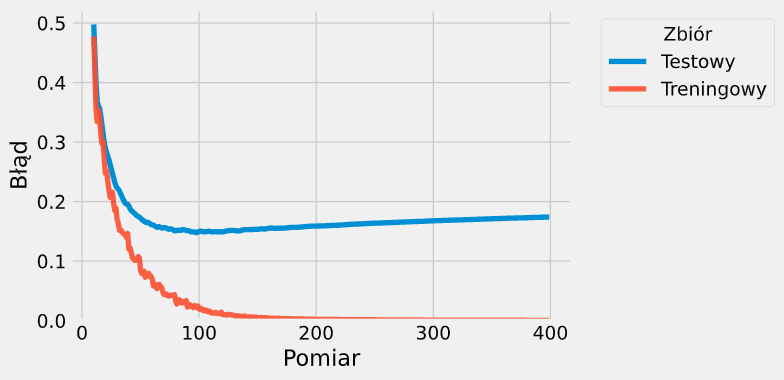
\includegraphics[width=\textwidth]{drop_err_0.png}
	\label{fig:res31}
\end{figure}
\begin{figure}[H]
	\centering
	\caption{Zachowanie funkcji błędu dla regularyzacji L2}
	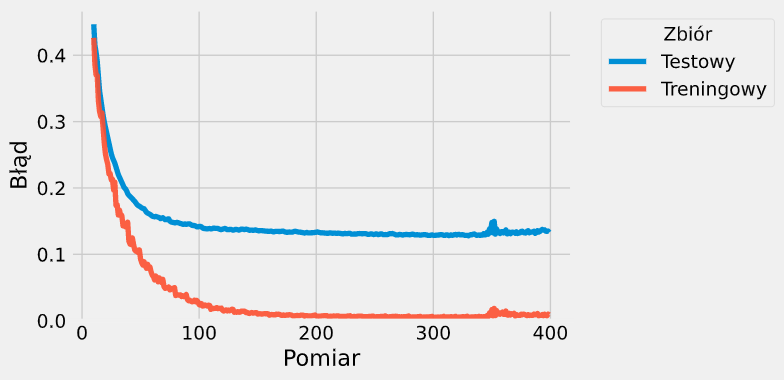
\includegraphics[width=\textwidth]{reg_err_l2.png}
	\label{fig:res32}
\end{figure}


\subsubsection*{Wnioski}
Na przedstawionym wykresie~\ref{fig:res32} można zaobserwować eliminację problemu przeuczenia, zaobserwowanego przy uczeniu bez regularyzacji (wykres~\ref{fig:res31}). Błąd testowy w przeprowadzonym eksperymencie stabilizuje się, a błąd treningowy nie osiąga 0, co sugeruje lepszą generalizację.

\newpage
\subsection{Wpływ regularyzacji łączonej L1 i L2 na przebieg procesu uczenia}
\subsubsection*{Założenia}
\begin{table}[H]
	\caption{Stałe dla eksperymentu 4}
	\label{tabela-const-4}
	\centering
	\begin{tabular}{lr}
		\toprule
		Parametr      & Wartość \\
		\midrule
		Regularyzacja & L1 L2     \\
		Lambda1       & 0.0001    \\
		Lambda2       & 0.0001    \\
		\bottomrule
	\end{tabular}
\end{table}

\subsubsection*{Przebieg}

Podczas eksperymentu model został zainicjalizowany 10 razy dla każdej z badanych wartości oraz wyuczony, uzyskane wyniki zostały zapisane w postaci pliku .plk do dalszej analizy.

\subsubsection*{Wyniki}
\begin{figure}[H]
	\centering
	\caption{Zachowanie funkcji błędu bez regularyzacji}
	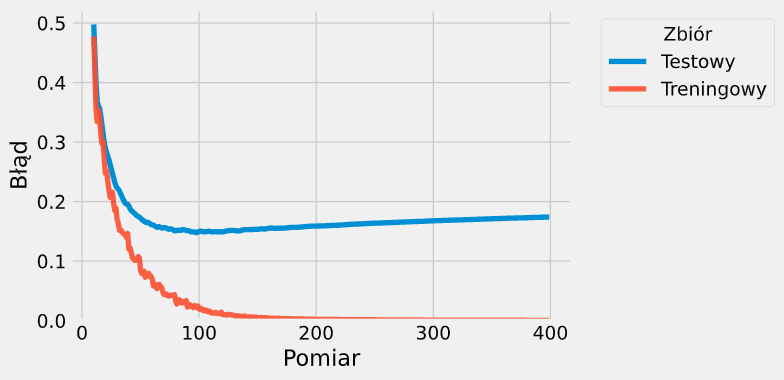
\includegraphics[width=\textwidth]{drop_err_0.png}
	\label{fig:res41}
\end{figure}
\begin{figure}[H]
	\centering
	\caption{Zachowanie funkcji błędu dla regularyzacji L1 L2}
	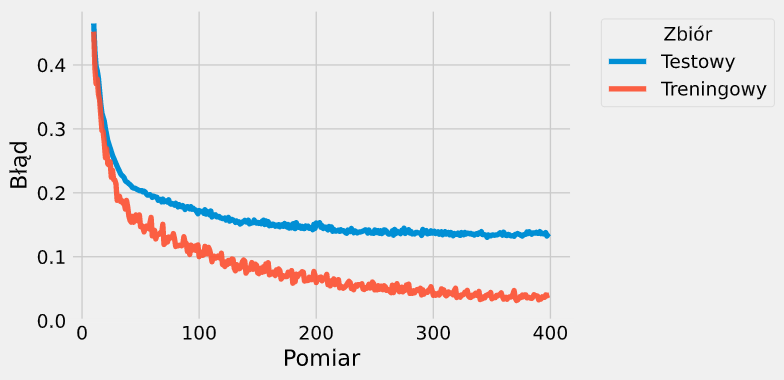
\includegraphics[width=\textwidth]{reg_err_l12.png}
	\label{fig:res42}
\end{figure}

\subsubsection*{Wnioski}
Na przedstawionym wykresie~\ref{fig:res42} można zaobserwować eliminację problemu przeuczenia, zaobserwowanego przy uczeniu bez regularyzacji (wykres~\ref{fig:res41}). Błąd testowy w przeprowadzonym eksperymencie nie przestaje spadać, a błąd treningowy nie osiąga 0, co sugeruje lepszą generalizację.

\newpage
\subsection{Porównanie metod}
\subsubsection*{Wyniki}
\begin{figure}[H]
	\centering
	\caption{Dokładność modelu w zależności od metody regularyzacji}
	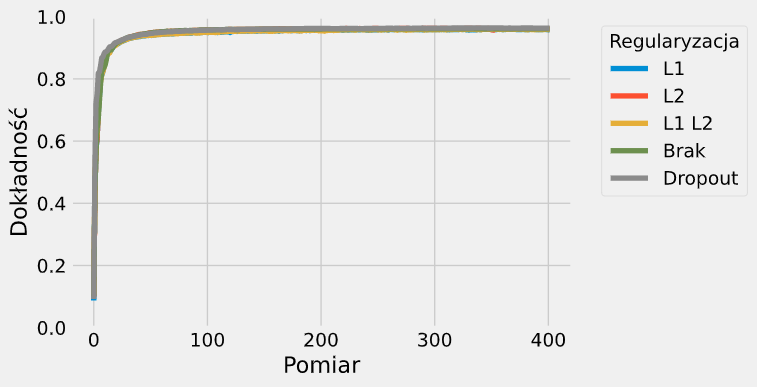
\includegraphics[width=\textwidth]{reg_acc.png}
	\label{fig:res51}
\end{figure}
\begin{figure}[H]
	\centering
	\caption{Dokładność modelu w końcowym etapie uczenia w zależności od metody regularyzacji}
	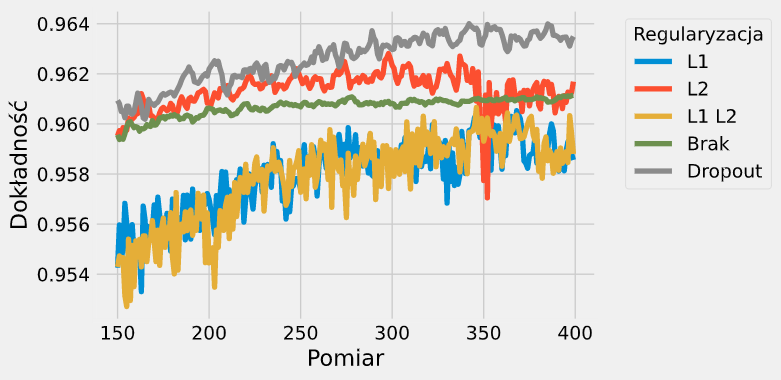
\includegraphics[width=\textwidth]{reg_acc_zoom.png}
	\label{fig:res52}
\end{figure}

\begin{table}[H]
	\caption{TODO}
	\label{tabela-res-51}
	\centering
	\begin{tabular}{rrr}
		\toprule
		Regularyzacja & Dokładność [\%] \\
		\midrule
		L1            & 96.34              \\
		L2            & 96.43              \\
		L1 L2         & 96.36              \\
		Brak          & 96.17              \\
		Dropout       & \textbf{96.58}     \\
		\bottomrule
	\end{tabular}
\end{table}

\subsubsection*{Wnioski}
Na przedstawionych wykresach~\ref{fig:res51} i~\ref{fig:res52} oraz tabeli~\ref{tabela-res-51} widać, że w przypadku rozpatrywanego zbioru danych zastosowanie regularyzacji nie dało znaczących zmian w dokładności modelu. Jednak każda z zastosowanych metod poradziła sobie w innym stopniu z problemem przeuczenia widocznym na wartościach funkcji błędu. Najgorsze wyniki dała metoda Dropout, która potrzebowała aż 80\% wyłączonych połączeń dla stabilizacji funkcji błędu, jednak przez fakt, że połączenia te są wyłączane w sposób losowy, trening takiego modelu trwał dłużej, co widać na wykresie~\ref{fig:res11}, gdzie sama dokładność zrównuje się z pozostałymi dopiero pod sam koniec procesu uczenia. Najlepsze efekty dały metody L1 oraz połączenie L1 i L2. Spowodowane jest to prawdopodobnie, popiera to też 80\% Dropout, tym, że warstwa ukryta złożona z 512 neuronów była zdecydowanie za duża i wyłączenie większości z nich dawało najlepszy efekt regularyzacyjny. Sama metoda L2 była w stanie ustabilizować funkcję błędu i zapobiec przeuczeniu.


\newpage
\section{Wnioski}

\begin{itemize}
	\item Zbyt skomplikowane modele mogą zbytnio przystosować się do danych uczących co negatywnie odbija się na ich generalizacji.
	\item Regularyzacja L1 pozwala na wyłączenie mniej ważnych połączeń w modelu co pozwala na jego zmniejszenie, a co za tym idzie przeciwdziałanie przeuczeniu.
	\item Regularyzacja L2 zmniejsza wartości wszystkich parametrów w modelu, jednak nie doprowadza ich do 0, co może być przydatne jeśli nie chcemy wykluczyć żadnych informacji.
	\item Regularyzacja pozwala na stosowanie większych modeli bez problemu przeuczenia.
\end{itemize}

\end{document}